\section{演化策略}
\label{sec:rs-es}

模拟退火只有一个状态，提议的形状事先给定。连续变量上还有一种选择：不维护候选，而维护一个“下一批候选从哪里抽”的分布，并让评价结果来修改这个分布。怎样根据一批候选的好坏，调整分布的中心、尺度和形状？这类方法称为\term{演化策略}（evolution strategy，ES）。

一代的流程是：抽出若干候选（称为\term{后代}，offspring），评价，选出较好的（称为\term{亲代}，parents），再由亲代决定下一代的分布。这里的“亲代”“后代”只是名称，所有内容都由下面的公式定义。本节用$\mu$表示亲代个数，$\lambda$表示后代个数，两者都是正整数，不再表示强凸常数和乘子。

\subsection{变异与重组}
\label{sec:rs-es-mutation}

后代从亲代而来。这一小节的问题是：单个后代怎样产生，有多个亲代时又怎样利用它们？

\paragraph{高斯变异}
从亲代$\bm{x}$产生后代的基本方式是加一个高斯扰动：
\begin{equation}
 \bm{y}=\bm{x}+\sigma\bm{z},\qquad\bm{z}\sim\mathcal{N}(\bm{0},\bm{I}),
 \label{eq:rs-mutation}
\end{equation}
称为\term{高斯变异}（Gaussian mutation）。步长$\sigma>0$控制扰动的整体尺度，各向同性指的是所有方向的扰动幅度相同。

用全卷的二次例子$f(\bm{x})=\tfrac12(x_1^2+9x_2^2)$手算一次。在$\bm{x}=(9,1)$处，$f=45$。取$\sigma=1$，抽到$\bm{z}=(-0.8,-0.5)$，后代是$(8.2,0.5)$，代价为
\[
 \tfrac12(67.24+2.25)\approx34.75,
\]
比亲代好，留下。抽到$\bm{z}=(-0.2,0.9)$时，后代是$(8.8,1.9)$，代价约为$54.97$，变差，丢弃。这样只保留变好的结果，就是最简单的$(1+1)$策略，名字的含义下一小节解释。

\paragraph{各向同性的局限}
这个目标在$x_2$方向比$x_1$方向陡$9$倍。图~\ref{fig:rs-es-isotropic}(a)在$(9,1)$周围取$\sigma=2$抽$60$个后代，绿点代价下降，红圈代价上升。圆形的云团和拉长的等高线不匹配：往$x_2$方向稍远一点就越出了等高线。

图~\ref{fig:rs-es-isotropic}(b)用$8\times10^5$个样本估计改善的概率。$\sigma$趋于零时，等高线局部接近直线，改善概率趋于$1/2$；$\sigma$增大，各向同性的抽样在$\sigma\approx2$时约为$0.31$，而沿等高线拉伸的抽样（两个方向的标准差比为$3:1$，面积相同）仍约有$0.42$。

\begin{BookInlineFigure}
 \centering
 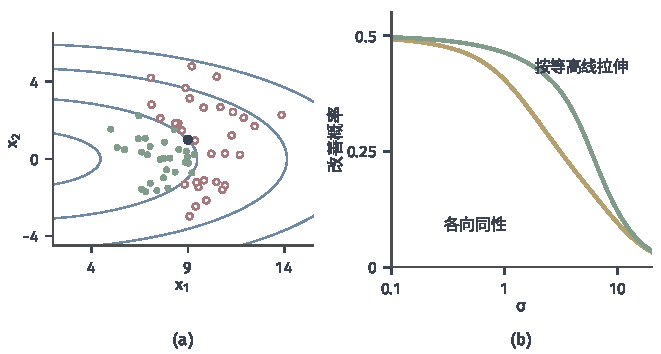
\includegraphics[width=112mm]{figures/05-optimization/05-stochastic-optimization/matplotlib/rs-es-isotropic/figure.pdf}
 \caption{$f=\tfrac12(x_1^2+9x_2^2)$上的变异，亲代在$(9,1)$。(a)蓝线是等高线，深色点是亲代，$\sigma=2$的各向同性后代中绿点改善、红圈变差。(b)改善概率随$\sigma$的变化，黄线为各向同性抽样，绿线的两个坐标标准差分别为$\sqrt3\sigma$和$\sigma/\sqrt3$，由固定种子抽样估计。}
 \label{fig:rs-es-isotropic}
\end{BookInlineFigure}

所以固定的圆形变异有两个问题：$\sigma$要随进展变化，形状也应当贴合地形。后面两小节分别解决。

\paragraph{多个亲代：选一个还是合成一个}
有多个亲代时，有两种产生后代的方式。一种是每次选一个亲代，在它周围变异。另一种是先把亲代合成一个点，称为\term{重组}（recombination），再从这一点变异，比如取权重$w_1\geq\cdots\geq w_\mu>0$，$\sum_iw_i=1$，按代价从好到差排序，
\begin{equation}
 \bm{m}=\sum_{i=1}^{\mu}w_i\bm{x}_{i:\lambda},
 \label{eq:rs-recombination}
\end{equation}
下标$i:\lambda$表示$\lambda$个后代中第$i$好的那个。

取两个亲代手算。$\bm{x}_{1:\lambda}=(7,-0.8)$的代价为$27.38$，$\bm{x}_{2:\lambda}=(8,0.6)$的代价为$33.62$。权重取$(3/4,1/4)$，重组后得到
\[
 \bm{m}=\tfrac34(7,-0.8)+\tfrac14(8,0.6)=(7.25,-0.45),\qquad f(\bm{m})\approx27.19.
\]
重组点比两个亲代都好。

原因在于两个亲代沿$x_2$的偏差一正一负，平均后相互抵消，$x_2$方向的代价又贵，于是抵消的好处很大。这是重组的一种效果：把各个亲代中互不相关的扰动平均掉，保留它们共有的移动。这也不是必然的结果，两个亲代偏差同号时重组就没有这个好处。

\paragraph{两类量}
演化策略中有两类量要分开。一类是\textbf{待优化变量}，就是候选$\bm{x}$本身，提交给$f$评价。另一类是\textbf{策略参数}，如$\sigma$和后面的协方差，它们决定怎样抽样，不提交给$f$，却随代更新。

\subsection{亲代选择}
\label{sec:rs-es-selection}

一代产生了$\lambda$个后代，下一代的亲代应从谁中选？这一小节比较两种规则，并说明它们各自能保证什么。

\paragraph{两种规则}
$(\mu+\lambda)$策略从$\mu$个旧亲代和$\lambda$个后代的并集中选出最好的$\mu$个。$(\mu,\lambda)$策略只从$\lambda$个后代中选最好的$\mu$个，旧亲代全部丢弃，因此要求$\lambda\geq\mu$；$\lambda=\mu$时全部后代都入选，就没有选择了，实际要取$\lambda>\mu$。

前面的$(1+1)$就是一个亲代、一个后代，留下较好者的规则。

\begin{theorem}[保留亲代时最好值不增]
\label{thm:rs-elitist}
设评价无噪声，亲代的代价是准确的。采用$(\mu+\lambda)$选择时，记第$t$代亲代中的最小代价为$f_{\min}^{(t)}$，则
\begin{equation}
 f_{\min}^{(t+1)}\leq f_{\min}^{(t)},\qquad t=0,1,\ldots.
 \label{eq:rs-elitist}
\end{equation}
\end{theorem}

\begin{proof}
第$t$代代价最小的亲代属于第$t+1$代选择的并集。选择取并集中最好的$\mu$个，所以并集的最小代价一定入选，而并集的最小代价不超过$f_{\min}^{(t)}$。
\end{proof}

\paragraph{这个保证的边界}
最好值不增不等于在进步，更不等于走向全局最优。把$(1+1)$规则放在双谷问题上，变异只提议左右相邻的状态，从$x=2$出发，两个邻居都更差，永远不会有后代入选。式~\eqref{eq:rs-elitist}成立，算法却永远停在$f=1$。

高斯变异的支撑是全空间，任何点都有正的概率被抽到，但一次跳过很宽的障碍的概率随距离指数下降，这个正概率在有限预算下没有意义。旧亲代保留也可能拖累搜索：一个特别好的旧亲代长期占据位置，后代都比不过它，$\sigma$的调整也因此失去依据。

\paragraph{两种规则的对比}
图~\ref{fig:rs-es-plus-comma}(a)在二次目标上用固定的$\sigma=0.5$，$\lambda=5$，$\mu=1$。保留亲代时曲线单调下降，到第$80$代代价约为$0.0026$。整代替换时，每一代的亲代都是新的，到了尺度$\sigma$能分辨的精度后就在附近上下波动，第$80$代当前代价约为$0.10$，只有其最好记录（虚线）约为$0.0016$。

图~\ref{fig:rs-es-plus-comma}(b)换到二维Rastrigin函数，$\sigma=0.45$，$40$次独立运行取中位数，起点$(2,2)$，代价为$8$。保留亲代时前期被小坑拦住，改进较慢；整代替换的最好记录（虚线）早期下降更快，因为当前点可以连续穿过小坑，但它的当前代价一直在$10$到$14$之间摆动，到$200$代时中位数约为$14$，而保留亲代的中位数约为$0.39$，整代替换的最好记录约为$0.85$。

\begin{BookInlineFigure}
 \centering
 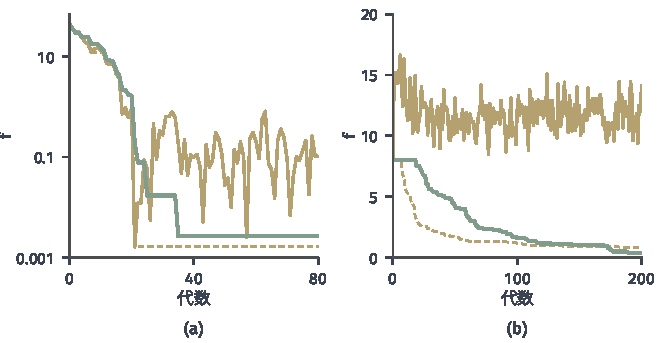
\includegraphics[width=112mm]{figures/05-optimization/05-stochastic-optimization/matplotlib/rs-es-plus-comma/figure.pdf}
 \caption{保留亲代（绿线）与整代替换（黄色实线为当前亲代的代价，黄色虚线为其历史最好）的对比，$\mu=1$，$\lambda=5$，$\sigma$固定。(a)$f=\tfrac12(x_1^2+9x_2^2)$，$\sigma=0.5$，一次运行，纵轴对数刻度。(b)二维Rastrigin函数，$\sigma=0.45$，$40$次运行的中位数，线性纵轴。}
 \label{fig:rs-es-plus-comma}
\end{BookInlineFigure}

\begin{BookInlineTable}
 \centering
 \caption{两种亲代选择的对比。}
 \label{tab:rs-plus-comma}
 \begin{tabular}{lll}
  \toprule
  & $(\mu+\lambda)$ & $(\mu,\lambda)$ \\
  \midrule
  旧亲代 & 与后代竞争 & 全部丢弃 \\
  无噪声时亲代最好值 & 不增 & 可能上升 \\
  是否需要单独保存最好记录 & 不必（已含在亲代中） & 必须 \\
  好亲代长期占位 & 可能 & 不会 \\
  \bottomrule
 \end{tabular}
\end{BookInlineTable}

两种规则都需要配合下面的尺度和形状更新。选择只决定谁留下，走多远、朝哪个形状抽，还要靠策略参数。

\subsection{协方差适应}
\label{sec:rs-es-cma}

圆形的抽样不贴合地形，这一小节的问题是：怎样让抽样分布的形状从评价结果中学出来？

\paragraph{主要思想}
把圆形的扰动换成椭圆形，后代从下式抽取：
\begin{equation}
 \bm{x}_i^{(t+1)}=\bm{m}^{(t)}+\sigma^{(t)}\bm{y}_i,\qquad\bm{y}_i\sim\mathcal{N}(\bm{0},\bm{\Sigma}^{(t)}),\quad i=1,\ldots,\lambda.
 \label{eq:rs-cma-sample}
\end{equation}
这里$\bm{m}^{(t)}$是分布的中心，$\sigma^{(t)}$是整体尺度，对称正定矩阵$\bm{\Sigma}^{(t)}$描述形状。\term{协方差矩阵适应演化策略}（covariance matrix adaptation evolution strategy，CMA-ES）的思路是：让“抽到好后代的那些位移”的分布，成为下一代的抽样分布。

好后代位移的方向多次出现，就说明沿那个方向走有好处，下次沿这个方向多抽一些。可以这样对应：等高线是一条拉长的山谷，中心$\bm{m}$是当前站立的位置，$\bm{\Sigma}$是下一次向四周探路时的步幅分配，把更多的步幅给谷底的走向。

具体的目标用旋转过的椭圆：
\begin{equation}
 f(\bm{x})=\frac12\bm{x}^\top\bm{A}\bm{x},\qquad
 \bm{A}=\begin{bmatrix}5&-4\\-4&5\end{bmatrix}.
 \label{eq:rs-rotated}
\end{equation}
$\bm{A}$的特征值是$1$和$9$，对应的特征方向是$(1,1)$和$(1,-1)$，所以山谷沿$(1,1)$方向。这种倾斜不能靠给两个坐标各设一个步长来表示，必须有非对角元。

更新分三步。第一步按评价排序，只用排序不用代价的数值，取前$\mu$个$\bm{y}_{i:\lambda}$。中心向它们的加权平均移动，权重$w_i$为正，和为$1$：
\begin{equation}
 \bm{y}_w=\sum_{i=1}^{\mu}w_i\bm{y}_{i:\lambda},\qquad
 \bm{m}^{(t+1)}=\bm{m}^{(t)}+\sigma^{(t)}\bm{y}_w.
 \label{eq:rs-cma-mean}
\end{equation}

第二步累积一条路径。一代的$\bm{y}_w$里有随机成分，但真实的好方向会在连续几代中重复出现。把连续几代的$\bm{y}_w$累加起来，得到\term{演化路径}（evolution path）：
\begin{equation}
 \bm{p}_c^{(t+1)}=(1-c_c)\bm{p}_c^{(t)}+\sqrt{c_c(2-c_c)\mu_w}\,\bm{y}_w,\qquad
 \mu_w=\frac{1}{\sum_iw_i^2},
 \label{eq:rs-cma-pc}
\end{equation}
其中$c_c\in(0,1]$决定记忆长度。$\mu_w$是有效亲代数，权重越平均越大。系数$\sqrt{c_c(2-c_c)\mu_w}$的来历在下一小节解释。

第三步更新协方差，把三部分加起来：
\begin{equation}
 \bm{\Sigma}^{(t+1)}=(1-c_1-c_\mu)\bm{\Sigma}^{(t)}
 +c_1\bm{p}_c^{(t+1)}\bigl(\bm{p}_c^{(t+1)}\bigr)^\top
 +c_\mu\sum_{i=1}^{\mu}w_i\bm{y}_{i:\lambda}\bm{y}_{i:\lambda}^\top.
 \label{eq:rs-cma-cov}
\end{equation}
第一部分是旧的形状，第二部分来自路径方向，称为秩一更新，第三部分是这一代选中位移的加权协方差，称为秩$\mu$更新。

式~\eqref{eq:rs-cma-cov}的$\bm{y}_{i:\lambda}$是相对旧中心的位移，用的是旧的$\bm{m}$。如果用新的$\bm{m}$，等于把这一代沿平均方向的进展减掉了，协方差就只记录了后代之间的散布，看不出朝哪边走有好处。

\paragraph{协方差保持正定}
抽样要求$\bm{\Sigma}$正定，下面的引理说明正权重时自动满足。

\begin{lemma}[协方差更新保持正定]
\label{lem:rs-cma-pd}
设$\bm{\Sigma}^{(t)}$对称正定，$c_1,c_\mu\geq0$，$c_1+c_\mu<1$，$w_i>0$。则由式~\eqref{eq:rs-cma-cov}得到的$\bm{\Sigma}^{(t+1)}$对称正定。
\end{lemma}

\begin{proof}
任取$\bm{u}\neq\bm{0}$，由式~\eqref{eq:rs-cma-cov}，
\[
 \bm{u}^\top\bm{\Sigma}^{(t+1)}\bm{u}
 =(1-c_1-c_\mu)\bm{u}^\top\bm{\Sigma}^{(t)}\bm{u}
 +c_1\langle\bm{u},\bm{p}_c^{(t+1)}\rangle^2
 +c_\mu\sum_iw_i\langle\bm{u},\bm{y}_{i:\lambda}\rangle^2.
\]
第一项为正，后两项非负。对称性由三个对称矩阵之和得到。
\end{proof}

这里假定权重全为正。有的实现给排序靠后的后代分配负权重，用来主动缩小不好的方向，那时要专门限制幅度，上面的引理不再适用。

\needspace{6\baselineskip}
\paragraph{变量}
下面用目标~\eqref{eq:rs-rotated}手算一代。要维护的量是：
\begin{itemize}
 \item $\bm{m}^{(t)}\in\mathbb{R}^n$：中心，$\sigma^{(t)}>0$：整体尺度；
 \item $\bm{\Sigma}^{(t)}\in\mathbb{R}^{n\times n}$：形状，对称正定；
 \item $\bm{p}_c^{(t)}\in\mathbb{R}^n$：协方差路径，$\bm{p}_\sigma^{(t)}\in\mathbb{R}^n$：步长路径，下一小节使用；
 \item 最好记录。整代替换时中心本身未必被评价过，记录必须单独保存。
\end{itemize}

\paragraph{初始化}
中心取$\bm{m}^{(0)}$，尺度取一个足以覆盖初始不确定性的量，形状取单位阵，两条路径取零。例中为了手算，把参数取成简单的数：
\[
 \bm{m}^{(0)}=\begin{bmatrix}3\\1\end{bmatrix},\qquad\sigma^{(0)}=1,\qquad\bm{\Sigma}^{(0)}=\bm{I},\qquad\bm{p}_c^{(0)}=\bm{p}_\sigma^{(0)}=\bm{0},
\]
\[
 \lambda=4,\quad\mu=2,\quad(w_1,w_2)=\bigl(\tfrac34,\tfrac14\bigr),\quad c_c=\tfrac12,\quad c_1=c_\mu=\tfrac15.
\]
于是$\mu_w=1/(9/16+1/16)=1.6$，路径系数$\sqrt{c_c(2-c_c)\mu_w}=\sqrt{1.2}\approx1.095$。此时$f(\bm{m}^{(0)})=13$。实际运行时参数按维数取默认公式，这里的简单数值只为演示。

\paragraph{每轮更新}
第$t$代依次执行以下步骤，直到预算用完或$\sigma$小到分辨不出差别。

\begin{enumerate}
 \item 由式~\eqref{eq:rs-cma-sample}抽$\lambda$个后代并评价，这一步要做$\lambda$次评价。例中$\bm{\Sigma}^{(0)}=\bm{I}$，取四个位移，后代和代价是
 \[
  \begin{gathered}
  \bm{y}_1=(-1,-0.6):\ \bm{x}_1=(2,0.4),\ f=7.2,\\
  \bm{y}_2=(0.5,0.5):\ \bm{x}_2=(3.5,1.5),\ f=15.25,\\
  \bm{y}_3=(-0.4,-1):\ \bm{x}_3=(2.6,0),\ f=16.9,\\
  \bm{y}_4=(1,-0.5):\ \bm{x}_4=(4,0.5),\ f=32.625.
  \end{gathered}
 \]
 \item 按代价排序，更新最好记录。例中顺序就是$1,2,3,4$，记录为$(2,0.4)$，代价$7.2$。
 \item 由式~\eqref{eq:rs-cma-mean}更新中心。例中
 \[
  \bm{y}_w=\tfrac34\begin{bmatrix}-1\\-0.6\end{bmatrix}+\tfrac14\begin{bmatrix}0.5\\0.5\end{bmatrix}=\begin{bmatrix}-0.625\\-0.325\end{bmatrix},\qquad
  \bm{m}^{(1)}=\begin{bmatrix}2.375\\0.675\end{bmatrix}.
 \]
 新中心的代价约为$8.83$，它没有被评价，这里只是核对。
 \item 更新步长路径$\bm{p}_\sigma$，见下一小节。
 \item 由式~\eqref{eq:rs-cma-pc}更新协方差路径。例中$\bm{p}_c^{(0)}=\bm{0}$，
 \[
  \bm{p}_c^{(1)}=1.095\,\bm{y}_w\approx\begin{bmatrix}-0.685\\-0.356\end{bmatrix}.
 \]
 \item 由式~\eqref{eq:rs-cma-cov}更新协方差。例中秩$\mu$部分是
 \[
  \tfrac34\begin{bmatrix}1&0.6\\0.6&0.36\end{bmatrix}+\tfrac14\begin{bmatrix}0.25&0.25\\0.25&0.25\end{bmatrix}=\begin{bmatrix}0.8125&0.5125\\0.5125&0.3325\end{bmatrix},
 \]
 秩一部分是
 \[
  \bm{p}_c^{(1)}\bigl(\bm{p}_c^{(1)}\bigr)^\top\approx\begin{bmatrix}0.469&0.244\\0.244&0.127\end{bmatrix},
 \]
 于是
 \[
  \bm{\Sigma}^{(1)}=0.6\,\bm{I}+0.2\,(\text{秩一})+0.2\,(\text{秩}\mu)\approx\begin{bmatrix}0.856&0.151\\0.151&0.692\end{bmatrix}.
 \]
 \item 更新$\sigma$，见下一小节。
\end{enumerate}

第一代结束，非对角元从$0$变成了正的$0.151$，大特征值$0.946$对应的方向约为$(0.86,0.51)$，已经朝山谷方向$(1,1)$倾斜了一点。最终在这一代得到中心$(2.375,0.675)$与记录$(2,0.4)$，后续各代重复以上步骤。

\paragraph{形状在做什么，以及它不是什么}
图~\ref{fig:rs-cma-adapt}取$n=2$的默认参数（$\lambda=6$，$\mu=3$）从$(5,-1)$出发。左图中椭圆起初是圆，几代之后沿山谷拉长，然后整体缩小。右图把$\bm{\Sigma}$的行列式归一后叠在一起：第$40$代的椭圆长短轴之比的平方约为$7.2$，方向与山谷一致，形状接近$\bm{A}^{-1}$的椭圆（比值为$9$）。

\begin{BookInlineFigure}
 \centering
 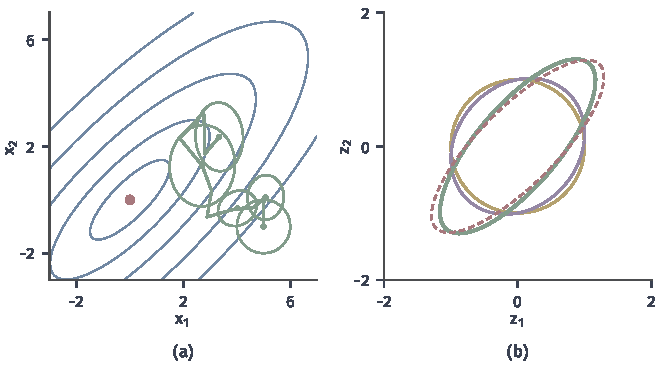
\includegraphics[width=112mm]{figures/05-optimization/05-stochastic-optimization/matplotlib/rs-cma-adapt/figure.pdf}
 \caption{CMA-ES在式~\eqref{eq:rs-rotated}上的一次运行，默认参数，$\lambda=6$，种子固定。(a)蓝线是等高线，绿线是中心的路径，绿色椭圆是第$0,2,4,7,11$代的$\sigma\bm{\Sigma}^{1/2}$单位圆像。(b)把$\bm{\Sigma}$的行列式归一化后的形状：黄线第$0$代，紫线第$6$代，绿线第$40$代，红色虚线是同样归一化的$\bm{A}^{-1}$。}
 \label{fig:rs-cma-adapt}
\end{BookInlineFigure}

在二次目标上，$\bm{\Sigma}$大致正比于$\bm{A}^{-1}$是可以理解的：作坐标变换$\bm{u}=\bm{A}^{1/2}\bm{x}$后等高线变成圆，而$\bm{\Sigma}\propto\bm{A}^{-1}$的抽样在$\bm{u}$坐标下正好是各向同性的。但这是对运行结果的描述，并不是一个无条件的等式。

一个简单的论证说明两者不可能恒等。CMA-ES只用排序，所以把$f$换成任何严格递增的函数，比如$h=\sqrt{f}$，排序完全不变，同一组随机数给出完全相同的$\bm{\Sigma}$序列。可是在$f>0$的点，
\[
 \nabla^2h=\frac{1}{2\sqrt{f}}\nabla^2f-\frac{1}{4f^{3/2}}\nabla f\nabla f^\top,
\]
它与$\nabla^2f$的形状不同。同一个$\bm{\Sigma}$不能同时是两者的逆。所以搜索协方差不是目标的Hessian，也不无条件地等于它的逆；它记录的是最近一段时间里选中位移的分布，并且依赖种群大小和有限的代数。

只用排序的好处恰恰在这里：算法的行为不随$f$的单调变换改变。这是它与第~\ref{chap:zeroth-order-optimization}章直接用函数值大小构造方向的做法的一个区别。

\subsection{步长适应}
\label{sec:rs-es-step}

协方差$\bm{\Sigma}$描述形状，而$\sigma$描述整体尺度。把两者分开的理由是：尺度需要比形状快得多的调整。这一小节的问题是：只看选中位移，怎样判断$\sigma$太大还是太小？

\paragraph{路径长度}
连续几代的位移如果彼此同向，说明本可以走得更远，$\sigma$偏小。如果彼此反向、互相抵消，说明走过了头在来回摆动，$\sigma$偏大。

图~\ref{fig:rs-cma-path-sigma}(a)(b)画的就是这两种情形：四段长度差不多的位移，同向时首尾相接的总位移很长，来回抵消时总位移很短。所以要比较的是累计路径的长度与“位移彼此无关时的路径长度”。

\begin{BookInlineFigure}
 \centering
 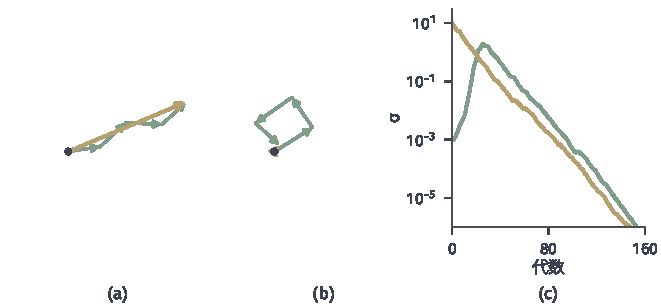
\includegraphics[width=112mm]{figures/05-optimization/05-stochastic-optimization/matplotlib/rs-cma-path-sigma/figure.pdf}
 \caption{路径长度与步长适应。(a)四段位移（绿）大致同向，累计位移（黄）长度约$4.8$。(b)四段位移互相抵消，累计位移长度约$0.2$。(c)五维球面$f=\tfrac12\lVert\bm{x}\rVert_2^2$上$\sigma$随代数的变化，只使用下面的步长路径，从$\sigma^{(0)}=10^{-3}$（绿）和$\sigma^{(0)}=10$（黄）出发，纵轴对数刻度。}
 \label{fig:rs-cma-path-sigma}
\end{BookInlineFigure}

\paragraph{标准化后累积}
为了把形状的影响除掉，累积之前先用$(\bm{\Sigma}^{(t)})^{-1/2}$把位移变成各向同性：
\begin{equation}
 \bm{p}_\sigma^{(t+1)}=(1-c_\sigma)\bm{p}_\sigma^{(t)}+\sqrt{c_\sigma(2-c_\sigma)\mu_w}\,\bigl(\bm{\Sigma}^{(t)}\bigr)^{-1/2}\bm{y}_w.
 \label{eq:rs-cma-psigma}
\end{equation}
再把路径长度与标准正态向量的期望长度比较，据此调整尺度：
\begin{equation}
 \sigma^{(t+1)}=\sigma^{(t)}\exp\Bigl(\frac{c_\sigma}{d_\sigma}\Bigl(\frac{\lVert\bm{p}_\sigma^{(t+1)}\rVert_2}{\mathbb{E}\lVert\bm{z}\rVert_2}-1\Bigr)\Bigr),\qquad\bm{z}\sim\mathcal{N}(\bm{0},\bm{I}).
 \label{eq:rs-cma-sigma}
\end{equation}
其中$d_\sigma>0$是阻尼。路径偏长时$\sigma$增大，偏短时$\sigma$减小。

系数的选取有一个清楚的理由。设选择完全随机，即排序与位移无关。这时$\bm{y}_w\sim\mathcal{N}(\bm{0},\bm{\Sigma}^{(t)}/\mu_w)$，于是$\sqrt{\mu_w}(\bm{\Sigma}^{(t)})^{-1/2}\bm{y}_w$是标准正态向量，记为$\bm{\xi}$。

若$\bm{p}_\sigma^{(t)}$也是标准正态向量，且与$\bm{\xi}$独立，那么式~\eqref{eq:rs-cma-psigma}的两项之和仍是高斯向量，协方差的系数为
\[
 (1-c_\sigma)^2+c_\sigma(2-c_\sigma)=1.
\]
所以随机选择下路径的分布不变，$\lVert\bm{p}_\sigma\rVert_2$的期望等于比较基准，$\sigma$在对数尺度上没有系统漂移。式~\eqref{eq:rs-cma-pc}的系数是同一个道理。一旦有真实选择，路径的长度偏离基准才来自评价信息。

\paragraph{例中的这一步}
接上一小节的第一代，取$c_\sigma=1/2$，$d_\sigma=1$，$\bm{\Sigma}^{(0)}=\bm{I}$，所以由式~\eqref{eq:rs-cma-psigma}，
\[
 \bm{p}_\sigma^{(1)}=1.095\,\bm{y}_w\approx\begin{bmatrix}-0.685\\-0.356\end{bmatrix},\qquad\lVert\bm{p}_\sigma^{(1)}\rVert_2\approx0.772.
\]

二维时$\bm{z}$的期望长度是$\sqrt{\pi/2}\approx1.253$。由式~\eqref{eq:rs-cma-sigma}，
\[
 \sigma^{(1)}=\exp\Bigl(\tfrac12\bigl(\tfrac{0.772}{1.253}-1\bigr)\Bigr)\approx\exp(-0.192)\approx0.825.
\]
路径比基准短，尺度缩小。第一代的路径从零开始，只积累了一代，这个判断偏保守。

图~\ref{fig:rs-cma-path-sigma}(c)是这个规则的效果。$\sigma$起初只有$10^{-3}$时，路径持续同向，$\sigma$在约$25$代内升到接近$2$；起初为$10$时，$\sigma$直接下降。之后两条线都随着接近最优点按稳定的比例减小，代价在$160$代后约为$10^{-13}$量级。

\paragraph{两条路径的职责}
两条路径形式相近，用途不同，表~\ref{tab:rs-two-paths}是对比。

\begin{BookInlineTable}
 \centering
 \caption{两条演化路径。}
 \label{tab:rs-two-paths}
 \begin{tabular}{lll}
  \toprule
  & 协方差路径$\bm{p}_c$ & 步长路径$\bm{p}_\sigma$ \\
  \midrule
  累积的量 & $\bm{y}_w$，含形状 & $\bm{\Sigma}^{-1/2}\bm{y}_w$，已标准化 \\
  用到它的什么 & 方向和符号相关 & 长度 \\
  更新谁 & $\bm{\Sigma}$（秩一项） & $\sigma$ \\
  \bottomrule
 \end{tabular}
\end{BookInlineTable}

\paragraph{更新顺序与数值处理}
一代内的次序是：抽样和评价；更新$\bm{m}$；用旧的$\bm{\Sigma}$更新$\bm{p}_\sigma$；更新$\bm{p}_c$；更新$\bm{\Sigma}$；最后更新$\sigma$。把$\bm{\Sigma}$的更新放在$\sigma$之前，是因为式~\eqref{eq:rs-cma-cov}中的$\bm{y}_{i:\lambda}$已按抽样时的$\sigma^{(t)}$标准化，这时不需要新的尺度。

实际实现还有一个小的修正：当$\lVert\bm{p}_\sigma\rVert_2$异常大，说明$\sigma$正在快速调整，这时暂停式~\eqref{eq:rs-cma-pc}右端的累积，防止形状被一次快速移动带偏。

代价方面，抽样要用$\bm{\Sigma}^{1/2}$，$\bm{p}_\sigma$要用$\bm{\Sigma}^{-1/2}$，这需要对称特征分解，稠密时一次约$O(n^3)$。通常每隔若干代才重新分解一次，把平均开销压到每次评价$O(n^2)$。

数值上要防止协方差病态：每次分解前把$\bm{\Sigma}$强制对称化，检查最小特征值是否仍为正，条件数太大时重置或停止。式~\eqref{eq:rs-cma-sigma}的指数形式保证$\sigma$恒正，无需额外处理。

\subsection{自然演化策略（补充）}
\label{sec:rs-es-nes}

前面的更新公式是逐条设计的。这一小节换一个角度：能不能把搜索分布的参数本身当作优化变量，直接写出它的梯度下降？这样得到的方法称为\term{自然演化策略}（natural evolution strategy，NES）。

\paragraph{分布参数上的目标}
设搜索分布$q_{\bm{\theta}}$由参数$\bm{\theta}$决定，把期望代价作为$\bm{\theta}$的函数：
\begin{equation}
 J(\bm{\theta})=\mathbb{E}_{\bm{x}\sim q_{\bm{\theta}}}[f(\bm{x})]=\int f(\bm{x})q_{\bm{\theta}}(\bm{x})\,\mathrm{d}\bm{x}.
 \label{eq:rs-nes-objective}
\end{equation}

$\bm{x}$可以是离散的，$f$可以不可微，只要$q_{\bm{\theta}}$对$\bm{\theta}$光滑。在可交换微分与积分的条件下，
\[
 \nabla_{\bm{\theta}}J(\bm{\theta})=\int f(\bm{x})\nabla_{\bm{\theta}}q_{\bm{\theta}}(\bm{x})\,\mathrm{d}\bm{x}.
\]

再把$\nabla q$写成$q\nabla\log q$，得到可以用样本估计的形式：
\begin{equation}
 \nabla_{\bm{\theta}}J(\bm{\theta})=\mathbb{E}_{\bm{x}\sim q_{\bm{\theta}}}\bigl[f(\bm{x})\nabla_{\bm{\theta}}\log q_{\bm{\theta}}(\bm{x})\bigr].
 \label{eq:rs-score-gradient}
\end{equation}
其中$\nabla_{\bm{\theta}}\log q_{\bm{\theta}}$称为\term{得分函数}（score function）。

\paragraph{与平滑估计的交叉}
取$q=\mathcal{N}(\bm{m},\sigma^2\bm{I})$，只把中心$\bm{m}$当参数，$\sigma$固定。写$\bm{x}=\bm{m}+\sigma\bm{z}$，得分是
\[
 \nabla_{\bm{m}}\log q=\frac{\bm{x}-\bm{m}}{\sigma^2}=\frac{\bm{z}}{\sigma}.
\]

代入式~\eqref{eq:rs-score-gradient}，有
\begin{equation}
 \nabla_{\bm{m}}J=\frac{1}{\sigma}\mathbb{E}_{\bm{z}}\bigl[f(\bm{m}+\sigma\bm{z})\bm{z}\bigr].
 \label{eq:rs-nes-gaussian}
\end{equation}
这里的$J$把$f$在$\bm{m}$周围按高斯权重做了平均，这正是第~\ref{chap:zeroth-order-optimization}章的高斯平滑目标，式~\eqref{eq:rs-nes-gaussian}正是那里的高斯方向估计。在这一实例上，分布梯度和平滑梯度是同一件事，这就是本节开头说的两种视角的重合。

一个可手算的例子：$f(x)=x^2$，$q=\mathcal{N}(m,\sigma^2)$，$m=2$，$\sigma=1$。这时精确值是$J=m^2+\sigma^2$，$\partial_mJ=2m=4$。取两个样本$z=\pm1$，读数为$f(3)=9$，$f(1)=1$，估计值为
\[
 \frac12\bigl(9\cdot1+1\cdot(-1)\bigr)=4,
\]
恰好是精确值。一般样本下估计值有方差，只有期望等于$2m$。

\paragraph{基线}
由于$\mathbb{E}[\nabla\log q]=\bm{0}$，给$f$减去一个常数$b$不改变期望，却改变方差。上例中估计量$(f(m+z)-b)z$的方差可以逐项算出。

记$a=m^2-b$，把$(m+z)^2-b$展开，估计量等于$az+2mz^2+z^3$，用$\mathbb{E}z^2=1$，$\mathbb{E}z^4=3$，$\mathbb{E}z^6=15$，奇数阶矩为零，得到
\[
 \operatorname{Var}=a^2+6a+15+8m^2.
\]

$m=2$时，$b=0$（$a=4$）的方差是$87$；$b=5$（$a=-1$）的方差是$42$；$b=7$（$a=-3$）的方差最小，是$38$。基线不改变估计的目标，只改变噪声大小。

\paragraph{自然梯度}
普通梯度依赖参数怎样写。把$\sigma$换成$\log\sigma$，梯度的方向就变了，可分布族是同一个。自然的办法是用分布之间的差别来度量参数的变化，即用\term{Fisher信息矩阵}（Fisher information matrix）
\begin{equation}
 \bm{F}(\bm{\theta})=\mathbb{E}_{\bm{x}\sim q_{\bm{\theta}}}\bigl[\nabla_{\bm{\theta}}\log q_{\bm{\theta}}(\bm{x})\nabla_{\bm{\theta}}\log q_{\bm{\theta}}(\bm{x})^\top\bigr]
 \label{eq:rs-fisher}
\end{equation}
作度量，沿\term{自然梯度}（natural gradient）下降：
\begin{equation}
 \bm{\theta}^{(t+1)}=\bm{\theta}^{(t)}-\eta\,\bm{F}(\bm{\theta}^{(t)})^{-1}\nabla_{\bm{\theta}}J(\bm{\theta}^{(t)}).
 \label{eq:rs-natural-gradient}
\end{equation}

一维高斯$\bm{\theta}=(m,\sigma)$，得分是$(z/\sigma,(z^2-1)/\sigma)$，由$\mathbb{E}z^2=1$，$\mathbb{E}(z^2-1)^2=2$，交叉项为$\mathbb{E}z(z^2-1)=0$，得
\[
 \bm{F}=\begin{bmatrix}1/\sigma^2&0\\0&2/\sigma^2\end{bmatrix}.
\]

还是目标$J=m^2+\sigma^2$，普通梯度是$(2m,2\sigma)$，自然梯度是
\[
 \bm{F}^{-1}\nabla J=(2m\sigma^2,\ \sigma^3).
\]
在$(m,\sigma)=(2,1)$，普通梯度是$(4,2)$，自然梯度是$(4,1)$。

图~\ref{fig:rs-nes-flow}比较两条连续轨迹。普通梯度沿直线同比例缩小$m$和$\sigma$。自然梯度下由$\mathrm{d}m/\mathrm{d}\sigma=2m/\sigma$得$m\propto\sigma^2$，均值比宽度收得快，分布先把中心挪到位，再缩小探索范围。

\begin{BookInlineFigure}
 \centering
 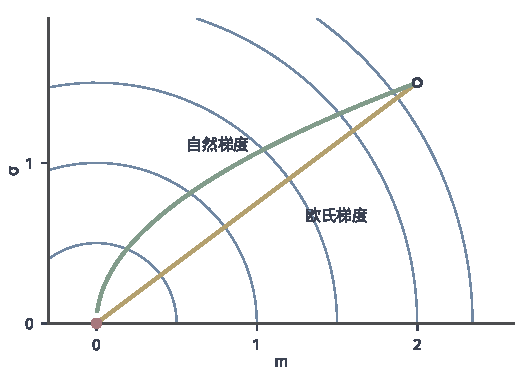
\includegraphics[width=88mm]{figures/05-optimization/05-stochastic-optimization/matplotlib/rs-nes-flow/figure.pdf}
 \caption{分布参数平面上的两条下降路径，$J(m,\sigma)=m^2+\sigma^2$，蓝线是$J$的等值线，空心圆是起点$(2,1.5)$，红点是最小点。黄线沿普通梯度，绿线沿自然梯度，后者满足$m\propto\sigma^2$。}
 \label{fig:rs-nes-flow}
\end{BookInlineFigure}

\paragraph{和CMA-ES的关系，以及要核对什么}
把$\bm{\theta}$限于中心，并把$f$换成按排序给的效用：选中的后代权重$w_i$，其余为$0$。对$\mathcal{N}(\bm{m},\sigma^2\bm{\Sigma})$，Fisher矩阵的均值块是$(\sigma^2\bm{\Sigma})^{-1}$，自然梯度下的均值更新量是
\[
 \sigma^2\bm{\Sigma}\cdot\sum_iw_i(\sigma^2\bm{\Sigma})^{-1}(\bm{x}_{i:\lambda}-\bm{m})=\sigma\sum_iw_i\bm{y}_{i:\lambda},
\]
这正是式~\eqref{eq:rs-cma-mean}。

这里有一点要小心：把$f$换成排序效用后，优化的已经不是原来的$J$，排序依赖当前样本，估计量也不再是式~\eqref{eq:rs-score-gradient}的无偏估计。基线只改变方差，排序效用改变了目标，把尺度参数写成$\sigma$还是$\log\sigma$则改变普通梯度的方向，这三件事不能混为一谈。说一个更新“是梯度下降”时，要先说清是哪个目标、哪个估计量、哪种度量。
